%!TEX root = ../../main.tex


\begin{figure}[p]
\centering
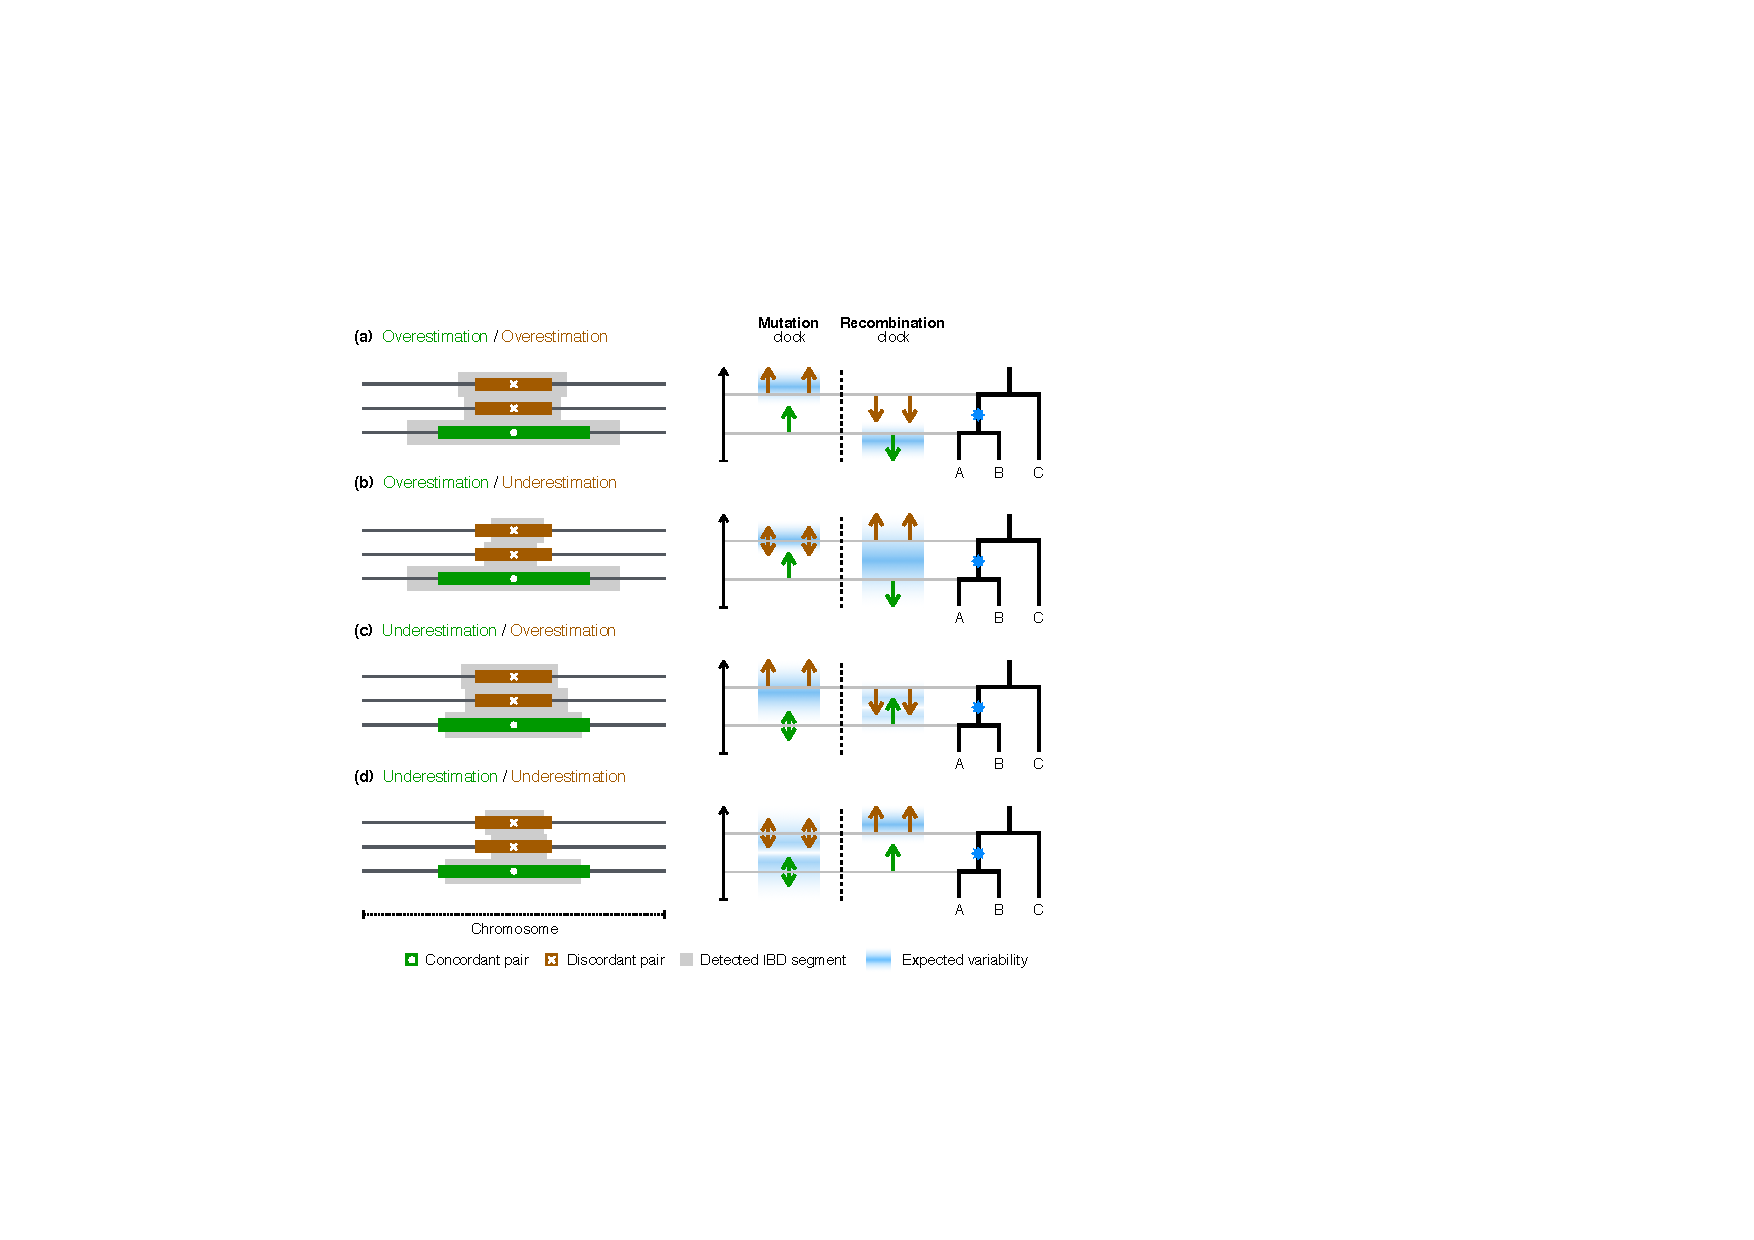
\includegraphics[width=\textwidth]{./img/ch5/info_age_bias}
\Caption{Expected estimation bias due to deficient IBD inference}%
{A minimal example is illustrated for a sample of \n{3} chromosomes where ${A,B \in X_c}$ and ${C \in X_d}$.
The focal mutation event is indicated in the genealogy of the sample (\emph{star}).
Each pair shares some haplotype region identical by decent, where the actual extent of the underlying IBD segment is shown for the concordant pair ${\{A,B\}}$ and the discordant pairs ${\{A,C\}}$ and ${\{B,C\}}$; indicated by \emph{green} and \emph{brown} bars, respectively.
The allele shared in concordant pairs is indicated (\emph{circle}), as well as the absence of allele sharing in discordant pairs (\emph{cross}).
Inferred IBD segments are shown as \emph{grey} bars at each true IBD segment, which may overestimate or underestimate the actual shared haplotype length.
Panels~\textbf{(a)} to \textbf{(d)} illustrate the possible cases of over and underestimation when observed in concordant and discordant pairs.
The arrows shown in relation to the times of coalescent events in the genealogy indicate the  direction to which the estimation under a given clock model is expected to tend, given the respective pattern of over and underestimation in concordant and discordant pairs.
The expected variability of the estimated age posterior distribution is indicated (\emph{blue}).
Note that only the mutation clock, \ClockM, and the recombination clock, \ClockR, are shown because \ClockC is a combination of both models.}%
{fig:info_age_bias}
\end{figure}
